\documentclass[a4paper,10pt]{article}

\usepackage[inner=3cm,top=3cm,outer=3cm,bottom=3cm]{geometry}
\usepackage[parfill]{parskip} % line skip between paragraphs instead of indents
\usepackage{fancyhdr}
\usepackage{fancyvrb}
\usepackage{graphicx}
\usepackage{xcolor}
\usepackage{setspace} % dynamic line spacing
\usepackage{hyperref} % automatic pdf bookmarks and hyperlinks
\usepackage{float} % picture placing
\usepackage{verbatim} % insert files verbatim
\usepackage[labelformat=empty]{caption} % picture captions
\ifxetex
  \usepackage{fontspec}
	% i xetex behövs inga fulhack för åäö
\else
	% åäö-hax för icke-xelatex
	\usepackage[utf8]{inputenc}
  \usepackage[T1]{fontenc}
\fi

% Header and footer
\pagestyle{fancy}\headheight 13pt
\fancyfoot{} % reset footer format
\fancyfoot[LE,RO]{\thepage}
\renewcommand{\headrulewidth}{0pt}
\renewcommand{\footrulewidth}{0pt}

% configuration
\def\thetitle{URD-2}
\def\groupname{The Meta Family}
\def\groupmembers{Daniel Bergström \\ Paulina Hensman \\ Marcus Hertz \\ Simon Karlsson \\ David Masko \\ Marcus Nordberg \\ André Nyström \\ William Perkola \\ Axel Riese \\ Kerry Zhang}
\def\version{Version 2.0}
\def\thedate{\today}
\renewcommand{\arraystretch}{1.2} % spacious tables

%----------------------------------------------------------------------------------------
%	TITLE PAGE
%----------------------------------------------------------------------------------------

\newcommand*{\titleGM}{\begingroup % Create the command for including the title page in the document
\hbox{ % Horizontal box
\hspace*{0.1\textwidth} % Whitespace to the left of the title page
\parbox[b]{0.75\textwidth}{ % Paragraph box which restricts text to less than the width of the page

{\noindent\Huge\bfseries \thetitle \\[0.5\baselineskip] \groupname}\\[2\baselineskip] % Title

{\large \version \\[\baselineskip] den \thedate}\\[2\baselineskip] 

\begin{doublespace}
{\Large \groupmembers} % Author name
\end{doublespace}

}}
\endgroup}


\begin{document}

% title page
\thispagestyle{empty}
\titleGM
\clearpage
\thispagestyle{empty}
\mbox{} % empty page for duplex
\clearpage 

% abstract
\thispagestyle{empty}
\section*{Sammanfattning} %unnumbered
Denna projektplaneringsrapport behandlar implementeringen av en SDK (Software development kit) till Android för applikationstestning.
\clearpage

% table of contents
% generated automatically
% from \section commands
\thispagestyle{empty}
\tableofcontents
\clearpage

% document change record
\setcounter{page}{1}
\section*{Versionshistorik}
% add to table of contents, but no numbering
\addcontentsline{toc}{section}{Versionshistorik}
\subsection*{0.1}
Första utkast. Varje underrubrik utom abstract är färdigskriven men texten är ej korrekturläst.

\subsection*{0.2}
Rapporten har uppdaterats med ett abstract.

\subsection*{1.0}
Alla delar är på plats. Gruppen anser att rapporten är färdig för inlämning.

\subsection*{1.1}
Mindre korrigering av källa.

\clearpage

\begin{flushleft} % left align
\section{Problembeskrivning}
\subsection{Detaljerad problembeskrivning}
Projektet framför oss består av att vi ska producera ett Software Development Kit (SDK) till vår projektgivare The Beta Family. Detta blir ett utvecklingsverktyg för applikationsutvecklare att direkt kunna få information från användaren om hur deras mobila applikation används och på så sätt få nödvändig information om hur de ska utveckla applikationer som är mer användarvänliga. Denna tjänst har redan fler än 9000 testare och har färdigställt tester för 2000 applikationer.


Tjänsten vi ska utveckla fungerar så att utvecklaren lägger upp sin applikation till The Beta Family och väljer den målgrupp som applikationen riktar sig mot, vilket operativsystem som används samt hur mycket personen som testar applikationen ska få i ersättning för att utföra detta test. Efter att testet är genomfört och testaren har rapporterat eventuella buggar och fel, betygsätts testaren av utvecklaren som betalar för testet.


Det erbjuds en SDK till iOS men inte till Android så projektet riktar sig till att utveckla en SDK för Android. Eftersom Androidmarknaden är mycket mer differentierad än vad den är på iOS-platformen så uppstår många fler utmaningar att lösa för att slutföra projektet. The Beta Family har även förbestämda krav och önskemål på hur projektet ska utvecklas och därför ger detta projektet en del ramar att hålla sig inom.


\begin{itemize}
	\item Android enheten ska ej behöva vara “rooted” vilket betyder att man inte ska behöva ha tillgång till alla processer i enheten utan det ska fungera med begränsad tillgänglighet som kan 	förekomma för normala Android användare.
	\item Projektets SDK ska vara byggd i Native Java.
	\item iOS versionen är väldigt enkel och tar endast 2 minuter att applicera och därför bör Android verionen också vara enkel att applicera.
	\item Inspelningen av skärmen ska ha en stadig bildfrekvens och är en av de första viktiga utmaningarna att testa för att se att projektet är möjligt.
	\item All beröring av enheten i form av tryck och fingerrörelser på skärmen ska markerar i grönt i enlighet med iOS versionen.
	\item Telefonens skärmstorlek samt position skall skickas vidare till servern.
	\item Användarens ansikte och röst skall spelas in och kan skickas in till servern som en separat video om det skulle behövas.
	\item Kan vi skapa references till OpenGL för att spela in t.ex. spel med en hög bilduppdatering?
	\item Hur spelar vi in vyer på tredjeparts SDK:er t.ex. för Google Maps?
\end{itemize}


Då detta är de grundläggande önskemålen och krav till SDK:n så ska detta utvecklas till Android och inte iOS vilket ger en del begränsningar som vi i projektgruppen inte kan komma förbi pågrund av skillnaderna mellan dessa plattformar. Problem som bra bildfrekvens från kameran är problem som inte går att komma undan. Detta är sådant som vi i projektgruppen har diskuterat och kommit fram till att begränsningarna är något vi inte kan göra något åt och är helt enkelt något vi får arbeta runt och göra en så bra lösning som möjligt.


När produkten är färdigställd så kommer den att bestå utav en “Front-end” som är det som kommer visas för användaren samt att ta in information från testaren samt utav “Back-end” som är den del som kommer att ta hand om och lagra all information som samlats in efter användning. “Front-end” skall byggas upp av HTML, CSS och JavaScript medan “Back-end” skall byggas upp i PHP med en databas i mySQL. \parencite{catalog}

\subsection{Motivering}
Alla gruppmedlemmar har ett stort intresse för teknisk utveckling och det är något vi alla vill arbeta med i framtiden. Det projekt vi valde reflekterar våra framtida ambitioner fast på en mildare nivå; att arbeta i grupp med att ta fram en teknisk lösning som skall levereras till ett företag (arbetsgivaren, The Beta Family i vårat fall) inom en given tidsram. Genom att prova på hur det är att jobba i grupp mot ett företag med ett projekt som faktiskt är tänkt att nå marknaden kommer vi att få erfarenheter som vi kommer kunna utnyttja i framtiden. Det är helt klart en fördel att känna till hur utvecklingsprocessen av en app går till när man som nyexaminerad civilingenjör når arbetslivet.

\subsubsection{Tekniska områden}

Projektet innefattar olika tekniska områden som tillsammans med kursens mål kommer att ge oss en inblick i hur projektarbete går till i arbetslivet. 
\begin{itemize}
	\item Androidprogrammering
	\begin{itemize}
		\item Back-end i form av inspelning av skärm, kamera, ljud och touch samt insamling av telefondata så som modell, skärmstorlek m.m.
		\item Front-end i form av ett intuitivt grafiskt användargränssnitt.
		\item Hur denna programvara kan integreras i appar som ska testas.
	\end{itemize}
	\item Datahantering; hur den insamlade datan från telefonen ska sammanställas, skickas och tas emot av en webbserver för att sedan presenteras i ett webbgränssnitt.
\end{itemize}

\subsubsection{Framtiden inom teknisk utveckling}
Den tekniska utvecklingen och i synnerhet mobiltelefoni har under de senaste åren gått framåt i rasande tempo. Fler och fler företag använder sig utav mobilappar för att nå ut till sina kunder med information, tjänster och produkter. Innan dessa mobilappar når marknaden måste de testas. Det som måste testas är tekniken bakom appen och användarvänligheten; hur den tänkta målgruppen reagerar när de använder appen. The Beta Family jobbar med att förmedla testare till apputvecklarna vilket vi tror starkt på eftersom appen kan nå en bredare grupp av testare från olika målgrupper och i mycket större skala än om utvecklarna testa appen själva.

\section{Bakgrund}
\subsection{Kommersiell bakgrund}
\subsubsection{The Beta Familys affärsidé}
The Beta Family har som affärsidé att bistå med testare när ett företag önskar betatesta sin smartphoneapplikation. Företaget får då erbjuda en belöning till varje testare som The Beta Family tar en andel av. Det samfund The Beta Family byggt upp gör att de kan erbjuda en mer sömlös betatestning jämfört med konkurrenter. TestFairy är ett företag med liknande affärsidé men där krävs det att utvecklarna själva har tillgång till testare då TestFairy enbart bistår med betatestnngsmjukvara. Genom en SDK för skärminspelning kommer testarna kunna bidra med bättre återkoppling vilket leder till att The Beta Family kan leverera en bättre tjänst för företagen.

\subsubsection{Konkurrens}
På grund av begränsningar i operativsystemet är det relativt få som försökt sig på att lansera en skärminspelare till Android. Det är först i den senaste versionen utav Android som möjligheten att spela in vad som händer på skärmen finns och då endast i utvecklingssyfte \parencite{kitkat}. Det krävs att mobilen är kopplad till en dator via USB och detta är främst tänkt att användas för att göra instruktionsfilmer och dylikt.

\subsubsection{TestFairy}
\label{testfairy}
TestFairy är ett företag med en affärsidé som påminner om den The Beta Family har. Målet är att underlätta betatestning av Androidapplikationer. Genom att använda sig av deras lösning kan man få en video som visar hur användaren navigerar i appen, grafer över diverse intressanta data (Exempelvis minnes- och CPU-prestanda), samt en mängd metadata.

Problemet med att Android inte har stöd för skärminspelning löser TestFairy genom att ta en skärmdump en gång i sekunden. Detta resulterar dock i en video som snarare påminner om ett bildspel än en rullande video. Dessutom förlorar man information om hur användaren reagerar på ljud från appen. Den visar dock det väsentliga användaren håller på med och ger i det stora hela en god överblick över hur appen används.

Jämfört med The Beta Family verkar TestFairy vilja fokusera mer på den tekniska aspekten utav en app. Fokus ligger på att finna  prestandaproblem snarare än att hitta problem i människa-dator-interaktionen. 

TestFairys betatestning går till som så att man laddar upp sin .apk-fil\footnote{Installationsfilen för applikationen}, väljer vilka testare man vill skicka ut till och sedan väntar man på resultatet. Detta underlättar för utvecklaren som inte behöver oroa sig över hur man implementerar TestFairys SDK\footnote{The Beta Familys iOS-testning förlitar sig på att utvecklaren själv implementerar deras SDK} men en nackdel är att TestFairy inte har en krets med testare. The Beta Family har i dagsläget cirka 9 000 testare medan man i TestFairys fall får förlita sig på att man känner tillräckligt många vänner som vill testa appen.

TestFairy riktar sig mot en internationell publik. All information finns på engelska och kärnan i den testdata man får ut är grafer som saknar språk. TestFairy skiljer sig dock från The Beta Family och Lookback i den mån att man inte själv måste veta hur SDK:n ska implementeras. En lägre kunskapsnivå krävs alltså av utvecklaren.

\subsubsection{Lookback}
\label{lookback}
Lookbacks lösning liknar på många sätt The Beta Familys. Företaget har i dagsläget bara stöd för iOS och är gratis under pågående betafasen\parencite{lookback}. Hur Lookback planerar att tjäna pengar framgår inte av deras hemsida. Till skillnad från TestFairy får testaren här möjlighet att filma sig själv medan hen använder appen och kan då komma med specifik återkoppling beroende på vad som händer på skärmen. The Beta Family har fortfarande en fördel i att man själv tillhandahåller testare medan Lookback förlitar sig på en tjänst vid namn TestFlight.

Själva betatestet presenteras på ett grafiskt tilltalande sätt. Varje testning (vilken Lookback kallar \emph{experience}) har en tidslinje som visar vilken del av appen de är i, etiketter på testet (såsom ``\emph{app flow}'', ``\emph{power user}'', m.fl), en vy som visar hur de navigerar runt i appen samt en video på användaren. 

Tjänsten är internationell i den mening att alla delar är på engelska. Inget hindrar dock testaren från att använda sig av sitt modersmål vid testning om detta är önskat av företaget. Eftersom Lookback främst riktar sig till utvecklare krävs en viss kunskapsnivå för att använda deras tjänst. Implementationen av SDK:n går snabbt och ska enligt utsago vara simpel men har man utvecklat en app kan det förutsättas att man är en avancerad användare med hyfsat goda kunskaper inom utvecklare.

\subsubsection{Diverse appar som kräver root-access}
\label{rootacc}
Det finns en mängd appar som möjliggör inspelning av mobilskärmen men dessa kräver root-access. Att skaffa root-access är något som kräver en viss kunskap och innebär en viss säkerhetsrisk då man låser upp hela mobilen, ungefär som ett adminkonto i Windows. Detta innebär att dessa appar är svåra att använda i betatestningssyfte då man som företag inte kan kräva att alla betatestare rootar sina mobiler. Dessutom är det oftast mer avancerade användare som rootar sina mobiler och i betatestning är sannolikheten stor att man inte bara vill ha återkoppling från avancerade användare. 

Eftersom dessa appar inte primärt är tänkta för betatestning går det inte uttala sig om deras lämplighet i sådana situationer. Appar har i regel inte tillåtelse att ta bilder av andra appars vyer så en app för betatestning skulle inte fungera utan det krävs någon form av SDK. Apparna utför en delmängd (skärminspelning) av det som detta projekt syftar genomföra men vissa delar (röstinspelning och kamerainspelning) saknas.

 Exempel på dessa appar är \emph{SCR Screen Recorder} \parencite{scr} och \emph{Screen Recorder} \parencite{sr}

\subsection{Teknisk bakgrund}
\label{subsec:tekniskbakgrond}
Målet med projektet är att utveckla en SDK åt Androidapplikationer och ett krav från arbetsgivaren är att koden ska vara ``native'', vilket innebär att utvecklingen kommer ske främst i Java, i Androids SDK. 

\subsubsection{Androidfragmentering}
Androidfragmentering syftar till det faktum att Androidplattformen körs i olika versioner på hundratals olika hårdvaruspecifikationer, och då måste skillnader i exempelvis skärmstorlek och tillgängliga bibliotek tas i hänsyn under utvecklingen. Ett av målen med projektet är just att ge applikationsutvecklarna möjligheten att fastställa att deras applikationer faktiskt fungerar som de är tänkta på de olika versionerna av plattformen. Under utvecklingsfasen för detta projekt kommer testning framförallt att utföras på emulatorer som bl.a. ingår i Androids SDK, eller som det finns separat programvara för, exempelvis Genymotion som har en gratis licens. I skrivandets stund (2014-02-15) är KitKat (version 4.4) den senaste Androidversionen, men 20\% av enheterna i cirkulation använder fortfarande Gingerbread (version 2.3.7).\parencite{androidversions} Endast 1,3\% använder en lägre version och Gingerbread är också den lägsta versionen som stöds av Genymotion. Allt detta har lett till beslutet att Gingerbread är den lägsta versionen som detta projekt kommer att stödja.

\subsubsection{Application Sandboxing}
\label{subsubsec:sandbox}
Androidarkitekturen implementerar ``application sandboxing'' vilket innebär att olika applikationer inte kan interagera med varandra direkt.\parencite{sandbox} Av denna anledning är det en SDK som behöver utvecklas som sedan kan integreras med applikationen som behöver testas. En fristående applikation skulle inte ha tillräckligt mycket behörighet för att spela in skärmen på den applikationen som ska testas. Denna sandboxing medför även att tredjepartens applikationer som tangentbord och Google Maps inte kan spelas in. 
Android har denna arkitektur på grund av säkerhetsskäl. En applikation som exempelvis har tillgång till tangentbordet skulle kunna registrera allt användaren skriver, vilket potentiellt skulle kunna inkludera lösenordet till dennes internetbank. 

\subsubsection{Metadata}
\label{subsubsec:Metadata}
I projektet ingår att samla in metadata om den mobiltelefon som testaren använder. Specifikt ingår i kravlistan att ta reda på testarens telefonmodell och skärmstorlek, samt kontinuerligt skicka med testarens skärmorientering. Det finns goda möjligheter att enkelt begära fram dessa data ur det officiella Android-API:t genom modulerna \textit{Build}, \textit{view.WindowManager} och \textit{app.Activity}. Åtkomst till dessa kräver endast grundläggande utvecklarbehörigheter \parencite{adoc}.

\subsubsection{Datapresentation}
\label{subsubsec:Datapresentation}
Insamlade data ska presenteras som ett flöde av information som gestaltar testarens användarmönster. Upprepade skärmdumpar ska tillsammans med testarens fingeravtryck bli till en video. Tillsammans med kamera- och ljudupptagning på testaren ska beställaren av testningen enkelt kunna bilda sig en uppfattning om hur produkten används.

Androids officiella API inkluderar en klocka med en upplösning på nanosekunder, \textit{System.nanoTime()} \parencite{adoc}. Klockan borde räcka gått och väl för att synkronisera kamera- och ljudupptagning med fingeravläsning och skärminspelning. Med samma klocka kan man trivialt spara tidsdata för varje skärmdump som tas, samt för varje fingerrörelse testaren gör. Man kan då representera testarens handlingar genom att ``måla över'' skärmdumparna med linjer som representarer fingerrörelser. Denna typ av enklare bildbehandlingsverktyg finns inbyggd i Android, i modulen \textit{Canvas} \parencite{adoc}. Dessa ihopslagna bilder kan sedan konverteras till en video med hjälp av den inbyggda modulen \textit{media.MediaCodec} \parencite{adoc}. Skulle det visa sig att \textit{media.MediaCodec} inte är kraftfull nog för våra ändamål finns även det fria alternativet \textit{ffmpeg} tillgängligt på Android \parencite{roman10}.

\subsubsection{Ljudinspelning}
\label{subsubsec:ljudinspelning}
Ramverket för multimedia stöder ljudinspelning med en rad olika ljudformat med klassen \textit{MediaRecorder}. Ljudformat och codecs som stöds är AAC LC, HE-AACv1, HE-AACv2, AAC ELD, AMR-NB, AMR-WB, FLAC, MP3, MIDI, Vorbis och PCM/WAVE \parencite{sound}.

\subsubsection{Kamerainspelning}
\label{subsubsec:kamerainspelning}
Tanken med kamerainspelning är att spela in användarens uttryck när denne testar applikationen. Android tillåter applikationer att spela in via frontkameran genom klassen \texit{MediaRecorder} \parencite{frontcamera} som nämnts ovan. Frontkameran har ett id-nummer som man spelar in ifrån.

\subsubsection{Rörelseinspelning}
Android har genom klassen \emph{view.MotionEvent}\parencite{motionevent} ett stort stöd för hantering av rörelser. Det är möjligt att få fram all information som kan tänkas vara intressant för detta projekt iochmed denna klass. Denna information måste behandlas så att den kan sparas undan på lämpligt sätt för att sedan läggas till ovanpå skärminspelningen.

\subsubsection{GUI}
\label{subsubsec:gui}
GUI för applikationen är mycket enkel och arbetsgivarnas önskan är att den ska vara så lik iOS-versionen som möjligt. Dubbeltryck med två fingrar drar ner en meny varifrån användaren kan välja att påbörja eller avsluta en inspelning, samt välja inställningar. Bland annat har användaren möjligheten att stänga av kamera- och ljudinspelning och trycksensorens färg kan väljas här. 

Ett alternativ för att skapa menyn är att använda en \textit{dialog}, vilket är ett popup-fönster vars innehåll kan skräddarsys \parencite{dialog}. 

Android har inte en inbyggd funktion för registrering av dubbeltryck med två fingrar, men klassen \textit{MotionEvent} samlar tillräckligt mycket information för att man ska kunna skriva en egen klass som kan avgöra om ett sådant dubbeltryck har skett \parencite{dbletap}.

Menyn ska vid visning glida in från skärmens övre del. Detta kan utföras med de inbyggda klasserna \textit{Animation} och \textit{TranslateAnimation}.

\subsubsection{Back- och front-end}
\label{subsubsec:backfront}
En back-end behövs för att ta emot datan som generas efter att en användare har betatestat en applikation och en front-end behövs för att presentera denna data för utvecklarna. Arbetsgivarna The Beta Family har redan en iOS-version av denna SDK med tillhörande back-end och front-end. Deras rekommendation är att det här projektet ska ha en egen miljö så att det inte uppstår ett beroende av deras kod, då data som generas i Android är annorlunda mot den som genereras i iOS. Dock bör samma ramverk som deras system är byggda på användas för att förenkla en senare integrering. Dessa ramverk är:

Back-end:
\begin{itemize}
	\item Ramverk: Laravel
	\item Språk: PHP, MySQL, JavaScript
\end{itemize}

Front-end:
\begin{itemize}
	\item Ramverk: Zurb
	\item Språk: HTML, CSS, JavaScript
\end{itemize}

\section{Riskbedömning}
\subsection{Ljudinspelning}
En potentiell risk för projektet är inspelningen från mikrofonen då ingen i gruppen har tidigare erharenhet av just detta. Vid närmare undersökning ser det dock inte ut som ett större hinder då ramverket för multimedia stöder ljudinspelning med en rad olika ljudformat med klassen MediaRecorder \parencite{sound} och det finns dessutom en steg-för-steg-guide på Androids utvecklarhemsida. Med gruppens samlade erharenhet av programmering anses därför ljudinspelningen vara en mindre risk. Av denna anledning har tidsåtgången för ljuinspelningen uppskattats till 5 timmar (se avsnitt \ref{sec:projektplan}).

\subsection{Inspelning av rörelser}
I den version av Screen Recorder som används till iOS syns testarens rörelser i videon. Eftersom iOS-versionen har andra förutsättningar som möjliggör en högre bilduppdateringsfrekvens blir rörelserna naturliga. Om det inte är möjligt att genomföra på Android finns det en risk i hur man vill lösa presentationen av rörelser. Antag att lösningen blir liknande den TestFairy använder, detta innebär i så fall att en bild visas per sekund. Visas bara en punkt där fingret befinner sig på varje bild blir det omöjligt att avgöra hur användaren rör sig runt i applikationen. Det behövs någon form av ``historia'' för rörelserna för att man ska kunna avgöra om testaren drar fingret, trycker eller sveper. Risken ligger inte lika mycket i den tekniska biten som i att gruppen måste komma överens om hur det ska presenteras.

\subsection{Skärminspelning}
I och med att skärminspelning inte är lika enkelt att utföra på Android som på IOS om man inte har tillgång till root finns risken att vi inte får så många bilder per sekund som vi önskar. TBF har meddelat att om det inte finns någon möjlighet att få en bra bildhastighet så räcker det med att få det lika bra som TestFairy. Bristen på erfarenhet av att skapa en screen-capture gör dock att det finns en risk att prestandan inte blir tillräckligt bra. I och med att detta anses vara en risk har det tagits i åtanke vid skapandet av planeringen.

\subsection{Kamerainspelning}
En annan teknisk utmaning är att spela in användarens ansikte med enhetens frontkamera. Android tillåter applikationer att spela in via frontkameran genom ett inbyggt bibliotek men eftersom att det så många olika enheter som använder Android är det inte säkert att inställningarna för att spela in från frontkameran blir desamma för alla enheter. Tanken är också att användarens ansikte automatiskt skall kännas igen vid kalibrering vilket kan bli en teknisk utmaning eftersom den inspelade videon måste behandlas i realtid för att känna igen ansikten.
\definecolor{Red}{rgb}{0.9,0.1,0.1}

\section{Projektplan}


\begin{center}
    \begin{tabular}{ | l | l | l |}
    \hline
    Rapporter & Deadline & Uppskattad tidsåtgång \\ \hline
    PPD-1 & v.8 (19/2) & 100h \\ \hline
    URD-1 & v.10 (5/3) & 100h \\ \hline
    ADD-1 & Kursens slut & 150h \\ \hline
    PPD-2 & Kursens slut & 50h \\ \hline
    URD-2 & Kursens slut & 50h \\ \hline
    \end{tabular}
\end{center}

(Deadlines är ungefärliga, eftersom det stod “i slutet av Mars” och liknande i handboken)

\begin{center}
    \begin{tabular}{ | l | l | l |}
    \hline
    Kod & Datum & Uppskattad tidsåtgång \\ \hline
    Mikrofon & 16/3 & 5h \\ \hline
    Kamera & 16/3 & 10h  \\ \hline
    Skärminspelning & 6/4 & 300h \\ \hline
    Touch & 16/3 & 10h \\ \hline
    Media & 4/5 & 300h \\ \hline
    Transfer & 4/5 & 200h \\ \hline
    Backend & 4/5 & 200h \\ \hline
    GUI & 16/3 & 50h \\ \hline
    \end{tabular}
\end{center}

\begin{center}
    \begin{tabular}{ | l | l | l | }
    \hline
    Övrigt & Deadline & Uppskattad tidsåtgång \\ \hline
    Möten & - & 260h \\ \hline
    Mötesprotokoll & - & 50h \\ \hline
    Demo & Början av Maj & 50h \\ \hline
    \end{tabular}
\end{center}

Till och med vecka 12 har vi två relativt tunga kurser parallellt med projektet. Därför räknar vi med att kunna lägga mindre tid på projektet då. Vi lägger mer fokus på rapporterna men ser till att bli klara med de lättare delarna av koden. 
\\\\
Vecka 13 och framåt kommer vi lägga mycket mer tid på koden. Vi börjar med att lösa skärminspelningen till den 6/4. Sedan behöver vi hitta ett sätt att komprimera vår media och fixa ett mindre backend-system att överföra inspelat data till. Till sist ska vi hitta en transfer-lösning. De sista punkterna kommer nog gå in i varandra en del, så vi ger alla samma deadline, 4/5, då all kod ska vara färdigställd. 
Därefter ska vi förbereda en presentation, skriva klart rapporter och presentera projektet. Rapporterna bör ha påbörjats parallellt med kodandet i April.
\\\\
Innan vecka 12 räknar vi med att kunna lägga runt 10 timmar per person och vecka på projektet, och efter vecka 12 räknar vi med 20 timmar per person och vecka.
DEADLINE för ALL KOD 4/5
Detaljerat schema: 

\begin{center}
    \begin{tabular}{ | l | l | l | l | l | l | l | l | l |}
    \hline
    Vecka & 4 & 5 & 6 & 7 & 8 & 9 & 10 & 11  \\ \hline
    Antal timmar & 100 & 60 & 70 & 110 & 100 &  &  &   \\ \hline
    Per person & 10 & 6 & 7 & 11 & 10 &  &  &   \\ \hline
    Händelser: & Föreläsningar & Föreläsning & Föreläsning & Föreläsning & Möte & Möte & Möte & Möte \\ \hline
    \end{tabular}
\end{center}

\begin{center}
    \begin{tabular}{ | l | l | l | l | l | l | l | l |}
    \hline
    Vecka & 12 & 13 & 14 & 15 & 16 & 17 & 18  \\ \hline
    \end{tabular}
\end{center}
\section{Genomförbarhetsstudie}
\subsection{Kravlista}
\subsubsection{Mobilen får inte vara ``rootad''}
Kravet att mobilen inte får vara ``rootad'' (förklarad i \ref{rootacc}) sänker dessvärre möjligheterna att kunna implentera en snabb och täckande skärminspelare. Utan ``root''-behörighet kan tredjepartsutvecklare inte komma åt den centrala grafiska modulen i Android \parencite{adoc}, och kan därför varken utnyttja systemets snabbhet eller kunna fånga en heltäckande bild av skärmen. Även om det tekniskt skulle vara mycket enkelt att släppa denna behörighet fri även från tredjepartsutvecklare, har Google gjort det klart att det inte ligger i deras intresse för närvarande \parencite{uhno}.

Detta gör att gruppen endast är förmögen att skriva en SDK som bara kan spara grafiken som hör till den testade applikationen. Exempelvis tangentbord, webbläsare och andra inbyggda systemmoduler verkar inte gå att fånga i nuläget. Även hastigheten kan komma att bli begränsad, i förhållande till vad som skulle vara möjligt med ``root''-behörighet. Troligen kommer prestanda och funktion att ha svårt att överskrida \textit{TestFairy}, som behandlas i \ref{testfairy}. Nöjar arbetsgivaren sig med den kvalitetsnivån är kravet dock genomförbart, då \textit{TestFairy} inte kräver någon ``root''-behörighet.

\subsubsection{Mjukvaran måste vara skriven i Java}
Alla gruppens medlemmar har gått samma introduktionskurs i datalogi, vilken till stor del behandlar språket java \parencite{inda}. Språket Java används som en grundsten i Android-plattformen, och Androids officiella API\footnote{Protokoll för ett program att kommunicera med andra program} är skrivet just i Java \parencite{adoc}. 

% TODO: citera föregående kapitel
Detta officiella API innehåller tillräcklig programkod för att spela in ljud och film, spara fingerrörelser över tid samt ta delvis täckande skärmdumpar. Med bakgrund av gruppmedlemmarnas erfarenheter i Java, samt de möjligheter som Androids Java-API erbjuder, kan kravet klassas som genomförbart.

\subsubsection{SDK:n måste vara enkel att integrera}
\subsubsection{Information som måste skickas med}
\subsubsection{Användarens ansikte och röst ska kunna spelas in}
\subsubsection{Informationen ska presenteras som ett tidsflöde}
\subsubsection{En serverapplikation som behandlar och presenterar datan}
\subsection{Sidouppgifter}
\subsubsection{SDK:n ska vara så lik iOS-versionen som möjligt}
\subsubsection{Tredjeparts-program ska kunna spelas in}
\subsection{Summering}

% references to be added
\renewcommand{\appendixtocname}{Appendix}
\renewcommand{\appendixpagename}{Appendix}
\begin{appendices}

\addcontentsline{toc}{section}{A Mötesprotokoll}
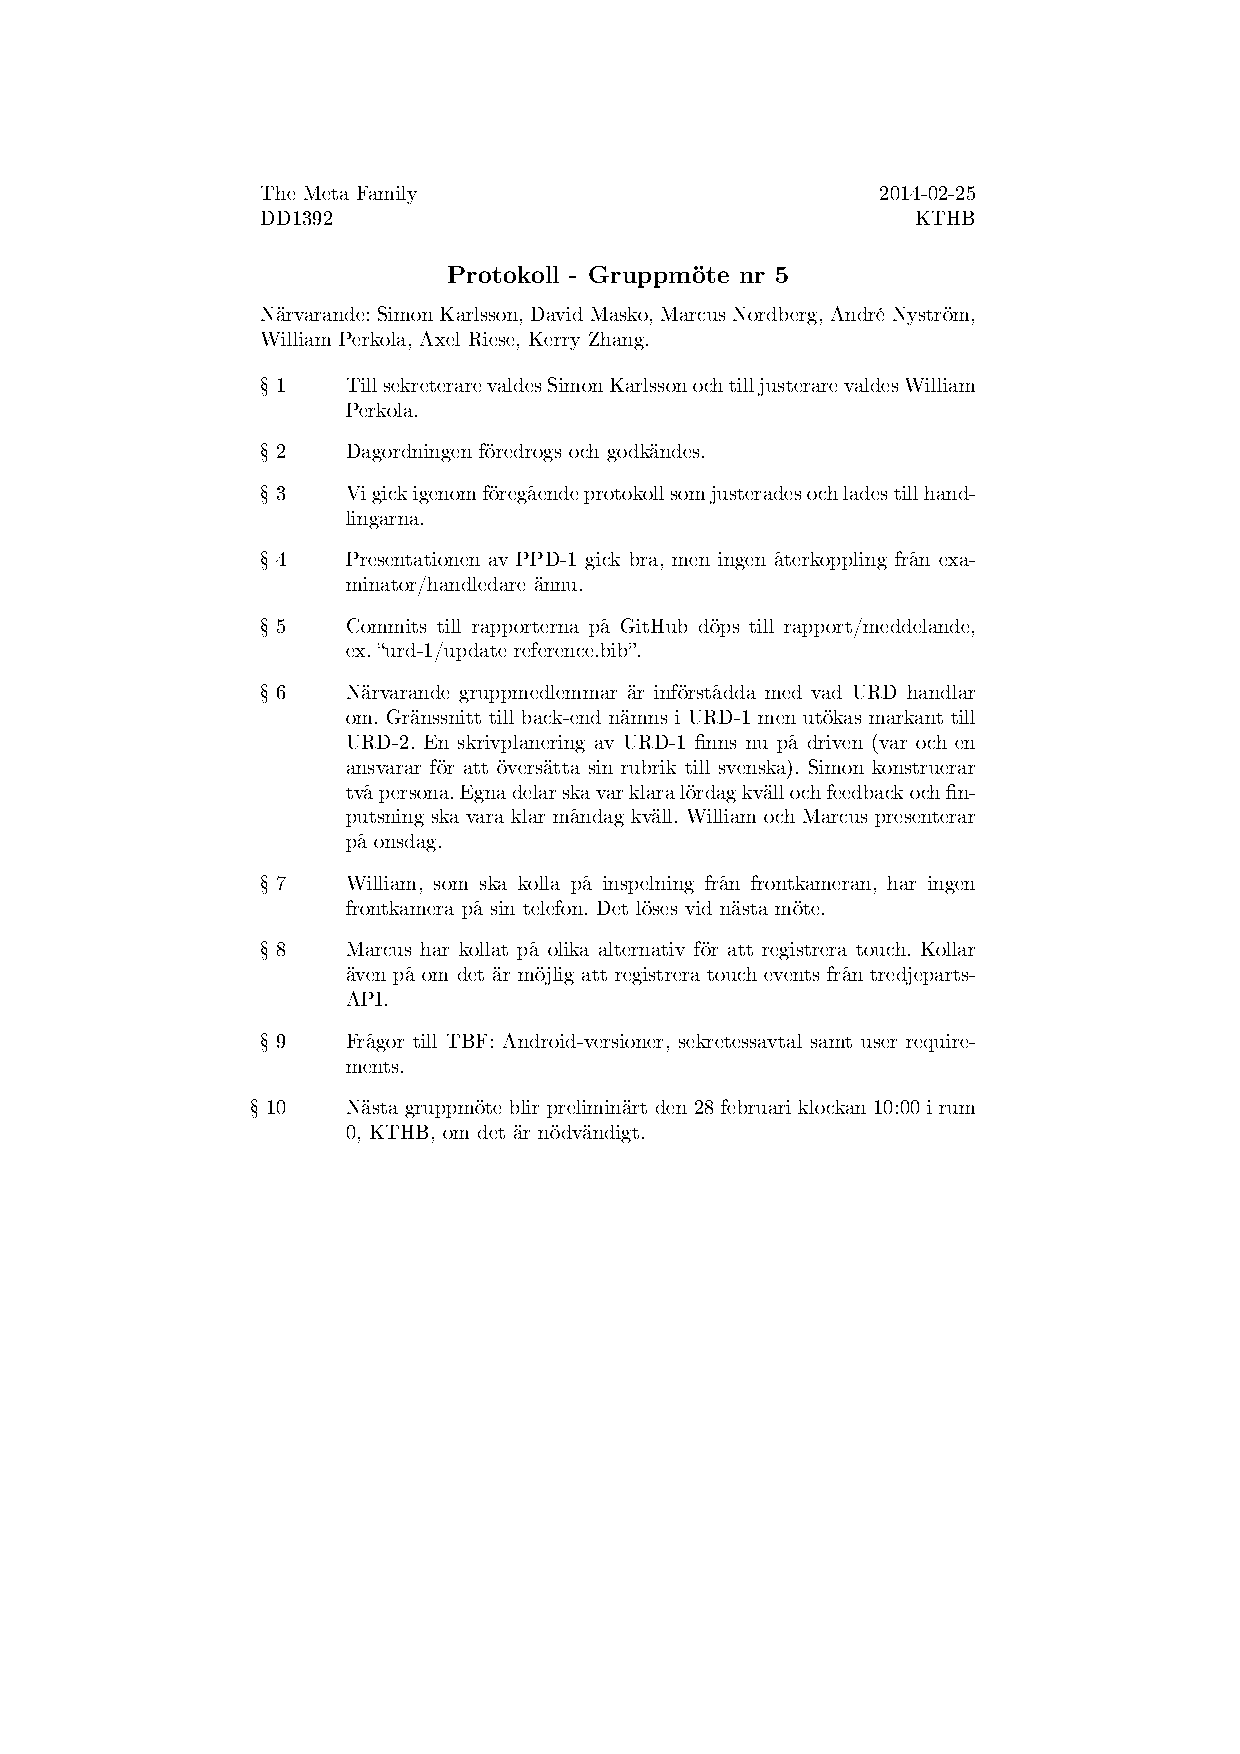
\includepdf{protokoll_2014-02-25}

\end{appendices}

\end{flushleft}
\end{document}
